\documentclass[conference]{IEEEtran}
\IEEEoverridecommandlockouts

\usepackage{cite}
\usepackage{amsmath,amssymb,amsfonts}
\usepackage{graphicx}
\usepackage{textcomp}
\usepackage{xcolor}
\usepackage{url}
\usepackage{booktabs} % For high-quality tables
\usepackage{hyperref}

\def\BibTeX{{\rm B\kern-.05em{\sc i\kern-.025em b}\kern-.08em
    T\kern-.1667em\lower.7ex\hbox{E}\kern-.125emX}}

\begin{document}

\title{Reinforcement Learning for Adaptive Traffic Signal Control on the Komitas Avenue}

\author{
\IEEEauthorblockN{Viktoria Melkumyan}
\IEEEauthorblockA{
\textit{American University of Armenia}\\
Yerevan, Armenia\\
Supervisor: Davit Ghazaryan
}
}
\maketitle

\begin{abstract}
Traffic congestions have become a widespread problem in Yerevan's major intersections. Current traffic light control systems, which operate with traditional fixed phase order and durations are unable to handle changing traffic scale during the day. This paper aims to discuss the use of Reinforcement Learning (RL) in traffic light signal control, aiming for an optimized traffic flow management, reduction of congestions and unnecessary waiting time, caused by pre-defined phase schedule. Komitas avenue with its 6 major intersections have been chosen, considering their importance for many urban routes, heavy traffic flow and connected nature of the intersections. Komitas network data has been modeled in SUMO (Simulation of Urban MObility) with manually collected real field data featuring order and duration of the phases, number of lanes and their connection for all intersections of interest. The work started with implementing a single-intersection controller and later expanded to developing the logic for decentralized, multi-intersection setup covering six junctions. The main contribution of this project is a realistic, field-grounded simulation framework that proves RL’s local effectiveness while actively identifying the need for inter-agent communication in urban corridor deployments.
\end{abstract}

\begin{IEEEkeywords}
Traffic signal control, reinforcement learning, SUMO, Deep Q-Network, adaptive traffic management, urban corridor, decentralized control.
\end{IEEEkeywords}

\section{Introduction}

Urban traffic congestion has become a widespread problem around the world over the years. In many cities, including Yerevan, traffic light management systems still rely on traditional approaches with fixed phase order and duration. While a static schedule might work adequately under perfectly average expected demand, it performs poorly when traffic patterns shift abruptly. For instance, heavy directional flow during the morning rush often faces the exact same green-time limits as completely empty cross-streets. This setup causes unnecessary delays, extended vehicle idling, and a highly inefficient use of overall road capacity.

Adaptive traffic signal control attempts to solve this inefficiency with Reinforcement Learning. Treating the intersection as a responsive environment, an RL agent can observe live network states and learn optimal phase-switching policies through continuous interaction.

This project focuses on the Komitas Avenue corridor in Yerevan. This area was selected specifically because it represents a dense, interacting chain of urban intersections with realistic geometric constraints. The main objective of this project is to construct an authentic SUMO (Simulation of Urban MObility) environment based on real observations, build a decentralized deep RL phase-selection framework, and evaluate its effectiveness. In order to determine if the agent actually succeeds in reducing congestion, the project monitors interconnected metrics such as average queue length, accumulated waiting time, trip duration, and time loss.

This work aims to answer two primary research questions:

\begin{itemize}
    \item Can a decentralized deep RL agent effectively outperform static schedules or simpler rule-based methods at a single, complex real-world intersection?

    \item How does the performance of decentralized RL control change in a dense multi-node urban corridor when the state representation and reward structure are redesigned for multi-intersection conditions?
\end{itemize}

\section{Literature Review}

Urban traffic management has changed a lot recently, moving from static schedules to data-driven models. We must look at traditional traffic control and highlight the exact areas where existing methods fail in order to understand whether reinforcement learning is a correct approach.

\subsection{Traditional and Actuated Traffic Control}
For decades traffic lights operated on fixed-time cycles based on historical averages. While simple to deploy, they fail completely during unpredictable events like accidents or sudden weather changes. To fix this, engineers introduced adaptive control systems such as SCOOT and SCATS \cite{b1}, \cite{b2}, which are still widely used today. These systems use hardware like inductive loop detectors to extend green lights when approaching vehicles are detected. While these systems represent a huge step forward from static timers, they rely on complex, human-designed logic trees. They essentially follow a set of "if-then" rules. As network complexity grows, manually tuning these parameters becomes incredibly tedious, and they often fail to find the globally optimal traffic flow because they are restricted by their hard-coded thresholds \cite{b2}.

\subsection{The Shift to Reinforcement Learning}
Because of the limitations of rule-based systems, researchers started experimenting Reinforcement Learning (RL), allowing the traffic controller to learn from trial and error \cite{b11}. Early studies in this area primarily used basic tabular algorithms like Q-learning. For example, IntelliLight demonstrated that deep reinforcement learning can dynamically adjust traffic light decisions based on traffic state information \cite{b3}.

However, tabular Q-learning becomes impractical as the number of possible traffic states increases. Modeling all possible queue-length combinations across multiple intersecting streets leads to an extremely large state space. The tables become too large to store or update efficiently. To solve this, recent literature has shifted almost entirely toward Deep Reinforcement Learning (DRL), where neural networks approximate the Q-values. Deep Q-Networks (DQN) have become the standard baseline for this task \cite{b4}. It makes sense why researchers prefer DQN; traffic signal control is naturally a discrete action problem (e.g., choose Phase 1, Phase 2, or Phase 3), which maps perfectly to the architecture of a DQN.

\subsection{Limitations in Existing RL Traffic Studies}
While deep learning has shown great results on paper, my review of the literature revealed a significant gap between academic simulations and real-world applicability. A major issue that repeatedly comes up is the oversimplification of the simulation environments. A vast majority of studies train their agents on idealized, symmetrical four-way intersections \cite{b5}, \cite{b6}. These models usually assume equal lane lengths, no turning restrictions, and identical speed limits. The reality of urban geography is rarely that neat. Because of not using authentic road topology, many existing papers overestimate how effectively their agents would perform in a real city.

Beyond the physical map geometry, there is also a noticeable trend where researchers overcomplicate the learning algorithm while ironically restricting the agent's actual flexibility. A number of recent studies fix the phase order and only allow the RL agent to adjust the \textit{duration} of each green light as a continuous time value \cite{b7}, \cite{b8}. Because the action space shifts from discrete choices to continuous ones (like outputting "stay green for 14.5 seconds"), these setups cannot use straightforward algorithms like DQN. Instead, they are forced to rely on heavy, continuous-action models like Soft Actor-Critic (SAC) \cite{b9}. While SAC is a highly capable algorithm for robotics, using it just to tweak traffic light timers often feels over-engineered. It requires intense hyperparameter tuning and massive computational overhead just to keep the training stable. Furthermore, by forcing a fixed phase order, these complex models still end up cycling through completely empty cross-streets, entirely missing one of the biggest real-world benefits of RL: the ability to dynamically skip unnecessary phases.

Another critical debate in the literature is the choice between centralized and decentralized multi-agent systems. When dealing with a corridor of intersections, centralized Multi-Agent Reinforcement Learning (MARL) attempts to control all traffic lights from a single "brain" that sees the entire network \cite{b10}. While this is mathematically optimal because it prevents intersections from working against each other, it is practically unrealistic. It requires massive computational power, perfectly reliable communication networks, and fails completely if one sensor goes offline.

On the other hand, decentralized agents are much easier and cheaper to deploy, but they introduce a problem known as non-stationarity \cite{b10}. Because each agent acts selfishly to clear its own local queue, it changes the traffic flow environment for its neighbors. For instance, clearing a massive queue at one intersection might suddenly flood the next intersection, causing a phenomenon known as "spillback." Some recent studies have tried to mitigate this by adding neighbor-state information into the agent's observation space \cite{b10}, but finding the right balance between local and network-level optimization remains an open challenge.

\subsection{Positioning of the Current Project}
This project aims to address the gap regarding environment authenticity and decentralized scaling. Rather than relying on a mathematically perfect grid, this work imports the exact geometric constraints of the Komitas Avenue corridor using OpenStreetMap data. By applying a standard DQN architecture to a real-world map, this project tests whether deep RL can handle genuine urban constraints without idealized assumptions.


\section{Methodology}

\subsection{Physical Observation Process}

I conducted an extensive physical field observation phase for the major corridor junctions: Gyulbenkyan, Vagharshyan, Papazyan, Vratsakan, Griboyedov, and Tigranyan.
Using stopwatches and visual inspection, I first mapped the physical lane discipline of the Komitas-Vagharshyan junction, identifying number of lanes, turning restrictions and lane-specific directional movements, as illustrated in Fig. \ref{fig:lane_discipline}. I then manually tracked the valid 5-phase signal sequences alongside their explicit green allocations and yellow transition buffer durations. These phase mappings are detailed in the grid provided in Fig. \ref{fig:phases_grid}. The same baseline data collection approach was used for the remaining 5 intersections.

\begin{figure}[htbp]
    \centering
    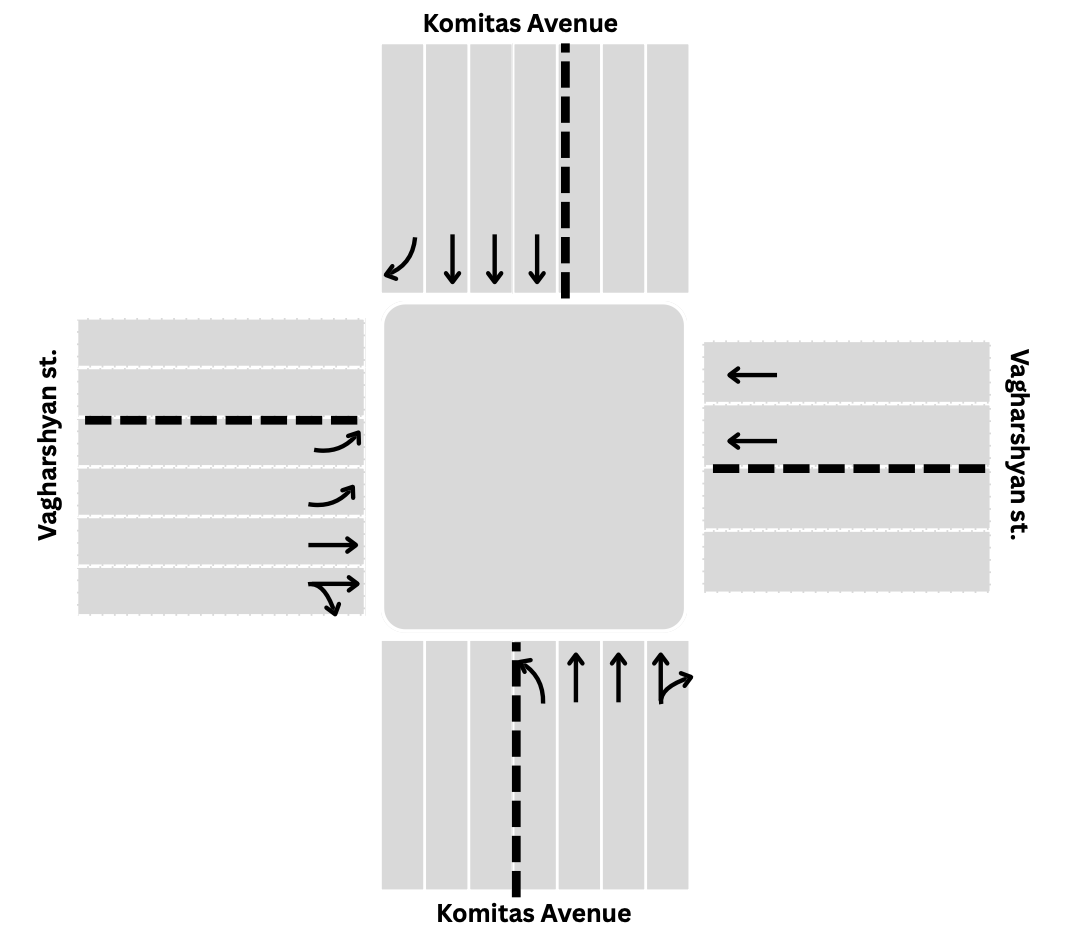
\includegraphics[width=0.45\textwidth]{img/lane_discipline.png}
    \caption{Intersection topology and lane discipline for the Komitas-Vagharshyan junction. Arrows indicate permitted turning movements per lane, serving as the physical constraints for the SUMO network edge routing.}
    \label{fig:lane_discipline}
\end{figure}

\begin{figure*}[htbp]
    \centering
    \begin{minipage}{0.32\textwidth}
        \centering
        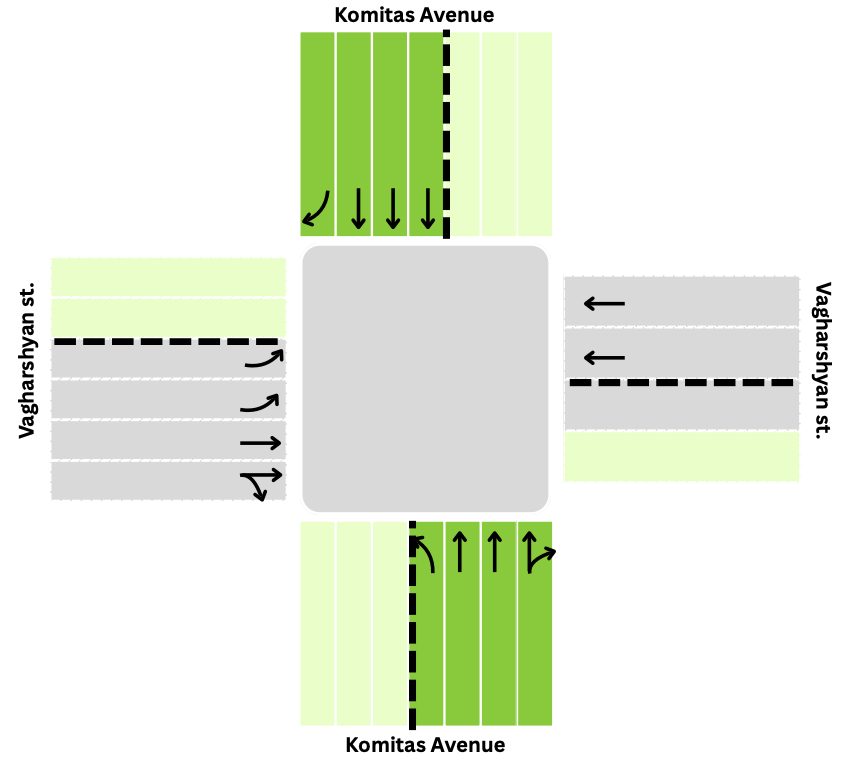
\includegraphics[width=0.8\linewidth]{img/phases/phase1.png} % Create cropped images!
        \caption*{Phase 1}
    \end{minipage}
    \begin{minipage}{0.32\textwidth}
        \centering
        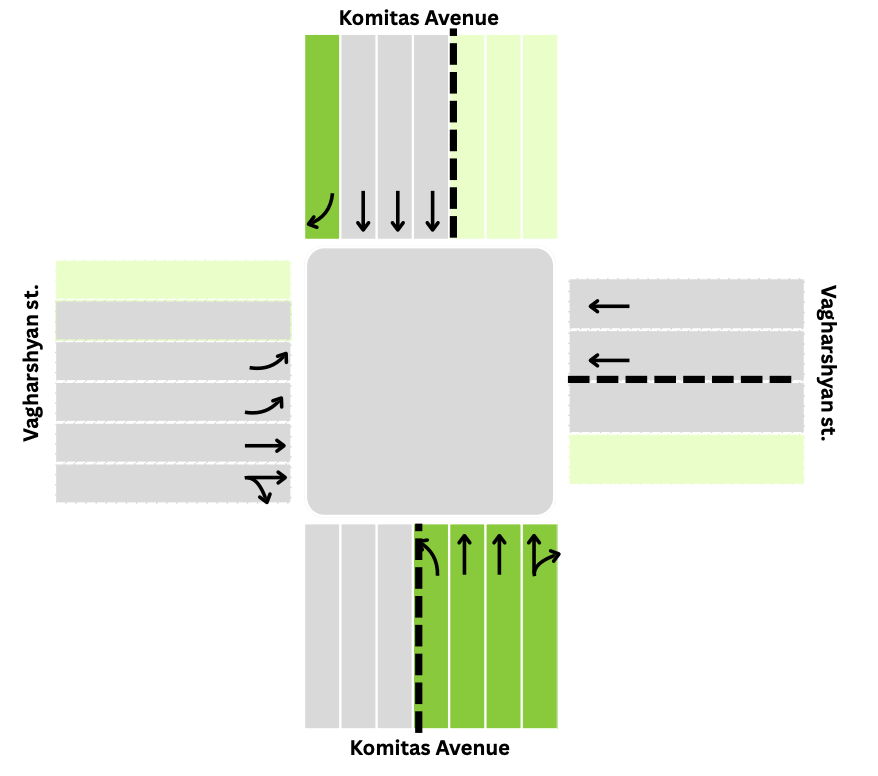
\includegraphics[width=0.8\linewidth]{img/phases/phase2.png}
        \caption*{Phase 2}
    \end{minipage}
    \begin{minipage}{0.32\textwidth}
        \centering
        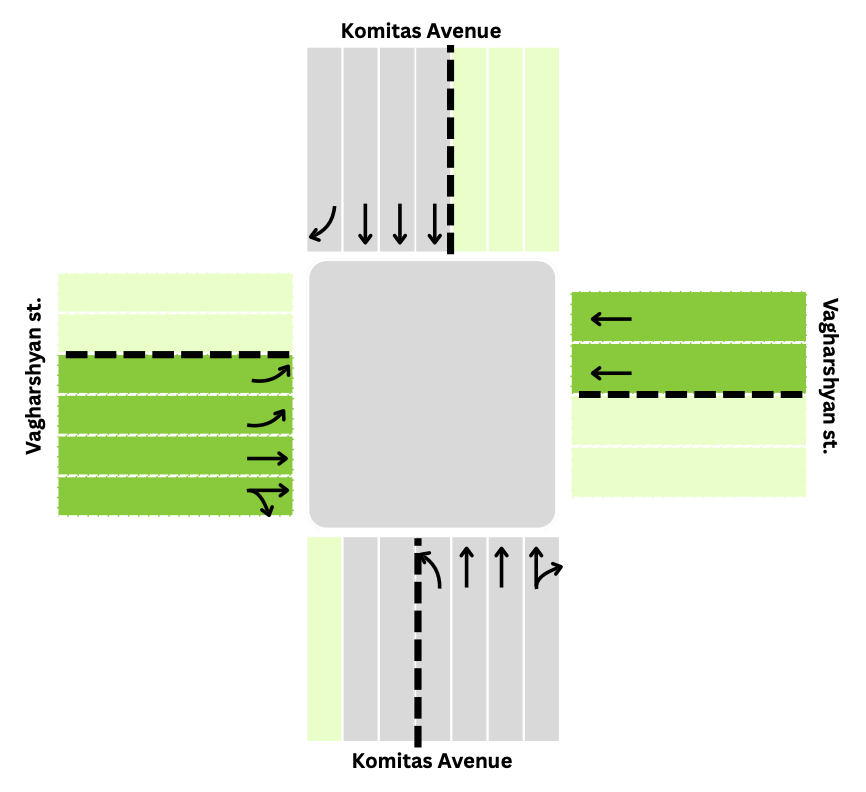
\includegraphics[width=0.8\linewidth]{img/phases/phase3.png}
        \caption*{Phase 3}
    \end{minipage}
    \vspace{0.2cm}
    \begin{minipage}{0.32\textwidth}
        \centering
        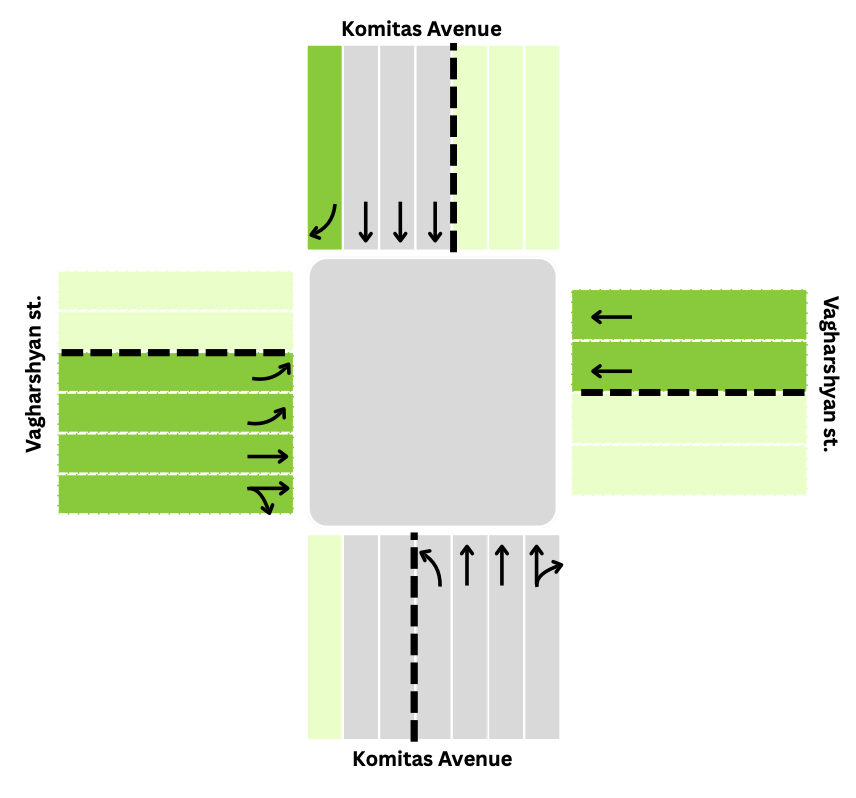
\includegraphics[width=0.8\linewidth]{img/phases/phase4.png}
        \caption*{Phase 4}
    \end{minipage}
    \begin{minipage}{0.32\textwidth}
        \centering
        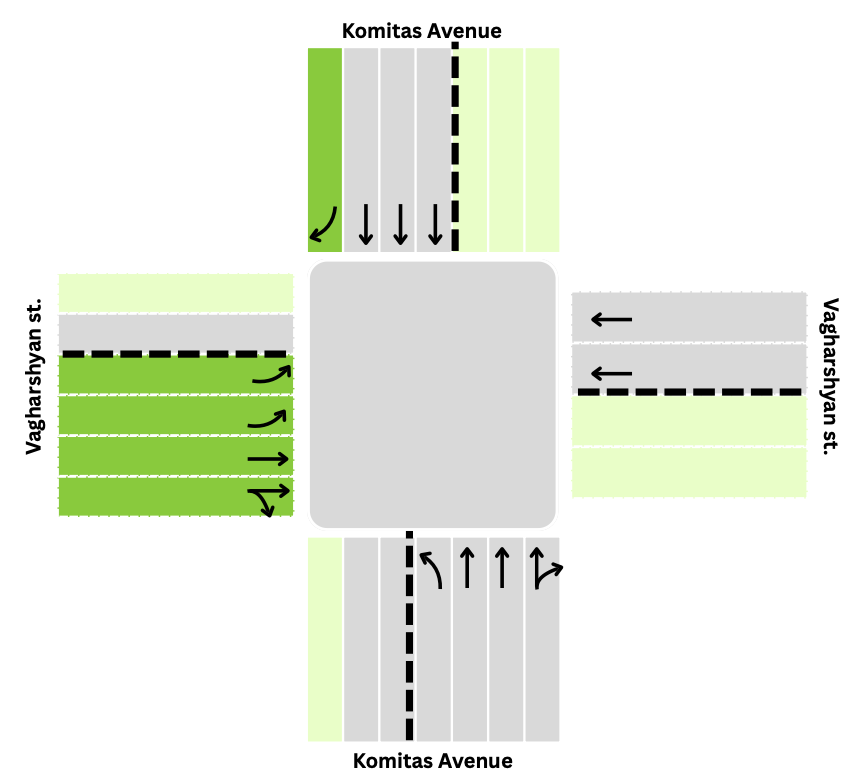
\includegraphics[width=0.8\linewidth]{img/phases/phase5.png}
        \caption*{Phase 5}
    \end{minipage}
    \caption{Field-recorded phase sequences for Komitas-Vagharshyan. Each phase was assigned a 3-second yellow transition buffer, establishing the logical baseline for the SUMO network.}
    \label{fig:phases_grid}
\end{figure*}

\subsection{Modeling in SUMO}
Komitas network data retrieved from Open Street Map (OSM) along with the manually collected parameters were transferred into the SUMO microscopic traffic simulation environment \cite{b12}. SUMO fits Armenian traffic conventions quite well at the infrastructure/rules level because Armenia follows standard right-hand traffic rules, which align with SUMO’s defaults.

\subsection{Preprocessing via NetEdit}
After careful visual inspection of Komitas network data model in SUMO, I revealed that the number of lanes for several intersections along with their movement direction and turning restrictions are not specified correctly. I used NetEdit, SUMO's graphical network editor, to modify road networks by adding missing lanes and removing unnecessary ones, that are not present in real Komitas network \cite{b12}. Additionally, during the OSM to SUMO conversion, I found that complex real-world intersections were often imported as clusters of independent junctions with each traffic light aimed to control separate lane connection. As shown in Fig. \ref{fig:netedit_process}(a), this fragmentation creates completely uncoordinated traffic light nodes.

To handle this, I merged these disjointed nodes into a single, unified junction (Fig. \ref{fig:netedit_process}(b)). Finally, as illustrated in Fig. \ref{fig:netedit_process}(c), I explicitly mapped and verified the internal lane connections—differentiating clear right-of-way flows from conflicting turn paths. This manual correction was necessary to ensure that one traffic logic controller accurately represented the entire physical intersection, guaranteeing valid vehicle paths down the corridor before any RL training began.

\begin{figure*}[htbp]
    \centering
    \begin{minipage}{0.32\textwidth}
        \centering
        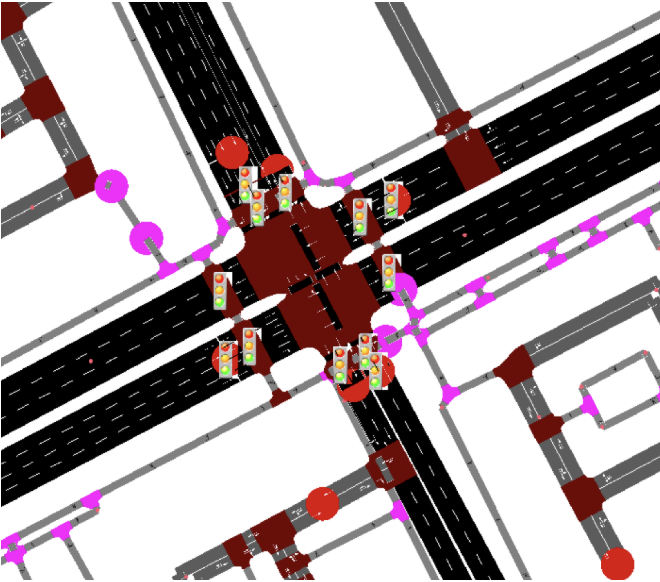
\includegraphics[width=\linewidth]{img/osm_messy.png}
        \vspace{0.1cm}
        \centerline{(a) Initial OSM Import}
    \end{minipage}\hfill
    \begin{minipage}{0.32\textwidth}
        \centering
        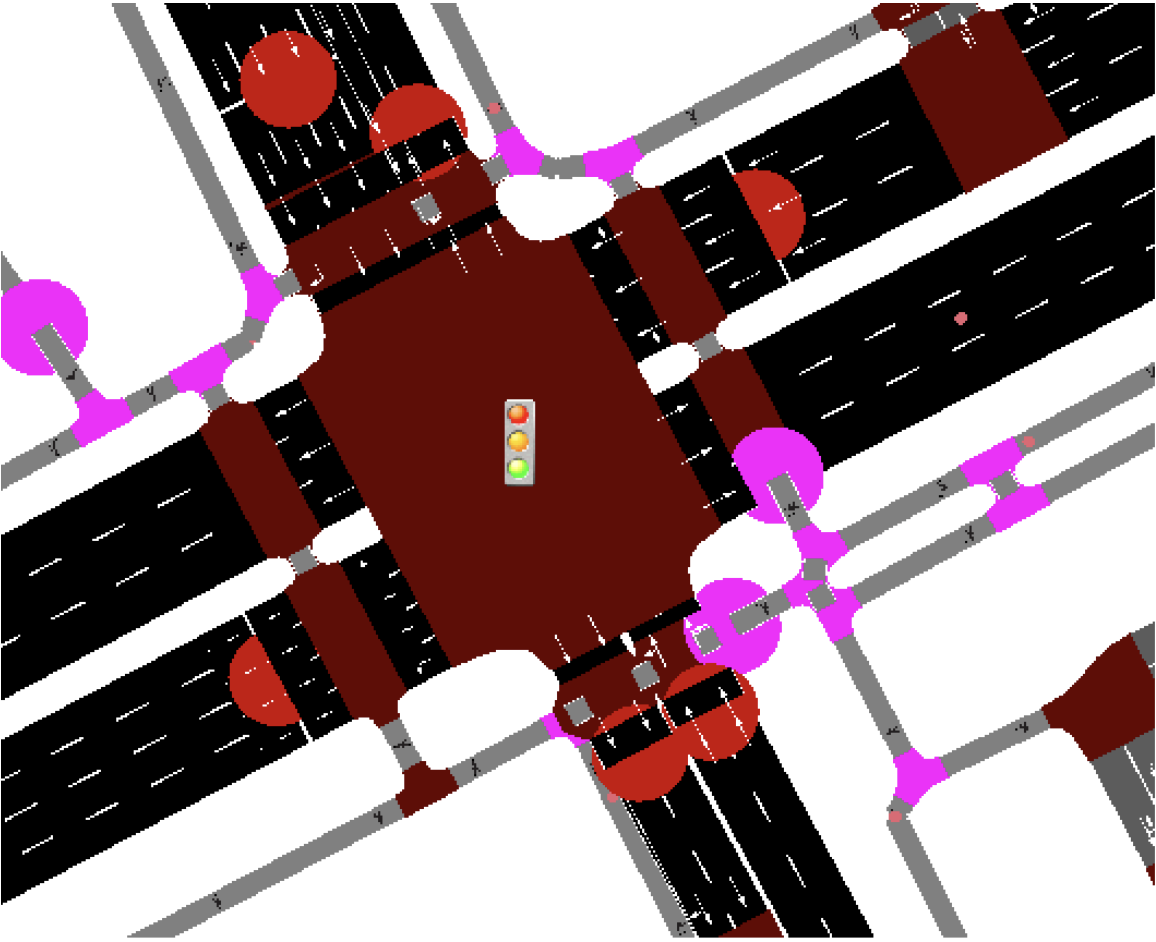
\includegraphics[width=\linewidth]{img/fixed_junction.png}
        \vspace{0.1cm}
        \centerline{(b) Consolidated Junction}
    \end{minipage}\hfill
    \begin{minipage}{0.32\textwidth}
        \centering
        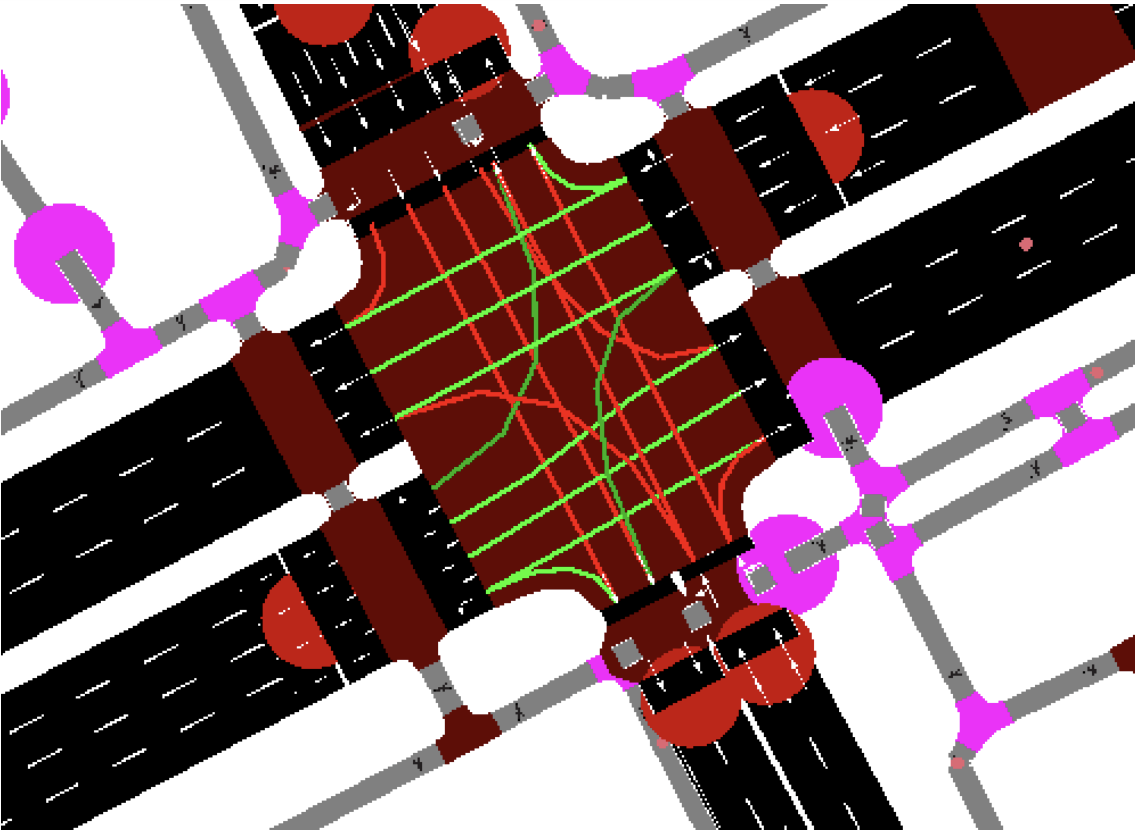
\includegraphics[width=\linewidth]{img/lane_connections.png}
        \vspace{0.1cm}
        \centerline{(c) Validated Lane Connections}
    \end{minipage}
    \vspace{0.2cm}
    \caption{The NetEdit network cleaning process for the intersections. (a) Default OpenStreetMap imports often fragment complex intersections into multiple unsynchronized traffic light nodes. (b) Fragmented nodes were manually collapsed to form a single, unified traffic signal controller. (c) Internal junction geometry and conflicting lane paths (green for clear paths, red for yielding/conflicting paths) were explicitly verified to guarantee realistic vehicle movement.}
    \label{fig:netedit_process}
\end{figure*}

\subsection{Traffic Demand Generation}
Synthetic demand scripts were built to stress-test the controller beyond average flow. Using a custom \texttt{generate\_traffic.py} pipeline interacting with SUMO's \texttt{duarouter}, I moved away from hardcoded routes to a probability-based portal entry system. Vehicles appear at the corridor boundary edges and navigate to varied exits with fixed speed.

The experiments utilize three main scenarios:
\begin{enumerate}
    \item \textbf{Off-Peak:} Lower baseline distribution (approx. 1,550 total generated vehicles) to ensure the controller doesn't overreact in empty environments.
    \item \textbf{Rush Hour:} High-density directional traffic simulating peak urban commuting conditions.
    \item \textbf{Corridor Stress:} Extreme probability settings pushing up to 8,500 vehicles across the simulation.
\end{enumerate}

\subsection{Reinforcement Learning Architecture}

\subsubsection{State Definition}
To make effective decisions, the RL agent requires a comprehensive but balanced view of the network. Omit crucial data, and the agent makes blind choices; give it too much raw data, and the neural network struggles to converge. The complete observation vector provided to each agent has a dimension of $N + 13$, where $N$ is the number of valid green phases at that specific intersection.

To bridge the gap between isolated control and corridor-level awareness, the features are grouped into four main categories:

\begin{itemize}
    \item \textbf{Phase and Timing Metrics ($N + 2$ features):} The agent observes the calculated queue pressure for each of its $N$ valid green phases (defined as incoming halted vehicles minus any downstream blockages). It also tracks the normalized elapsed time of the active green light and its index position (0 to 1) within the overall signal cycle.

    \item \textbf{Local Congestion Factors (3 features):} To evaluate immediate junction health, the state captures the total halted queue, the accumulated waiting time across all controlled lanes, and the ``worst-lane'' pressure. Tracking the maximum queue on a single lane is a deliberate inclusion to ensure the agent does not artificially inflate its score by permanently abandoning a minor side-street.

    \item \textbf{Downstream and Global Load (2 features):} The agent monitors immediate downstream spillback pressure. This is essential because a green light is practically useless if the exit lane is already full; this feature teaches the agent to hold a red light rather than jam an intersection. Additionally, it receives the total number of vehicles currently in the entire SUMO network, giving it a baseline sense of overall traffic density.

    \item \textbf{Neighbor Awareness (6 features):} To function effectively in the multi-node corridor without relying on a heavy centralized controller, the agent is given limited "line-of-sight" to its adjacent intersections. For both the previous and next neighbors, the agent observes their current queue pressure, spillback pressure, and phase position. This allows the local agent to anticipate incoming platoons and prepare its phases accordingly.
\end{itemize}

\subsubsection{Action Space \& Yellow Transition Logic}
Rather than relying on a single centralized controller, each of the six intersections operates its own local action space. For a junction with $k$ valid green phases, the action dimension is $1 + k$. Action 0 is always defined as \texttt{EXTEND}, which holds the current green light for an additional 5-second interval. All remaining actions correspond to direct switches to specific target green phases.

To keep the simulation physically realistic, I implemented dynamic action masking to enforce strict timing constraints. If a phase has been active for less than a 10-second minimum, all switching actions are masked out, forcing the agent to \texttt{EXTEND}. This prevents the agent from finding loopholes via dangerous, rapid signal flickering. Conversely, if a phase reaches the 90-second maximum limit, an immediate switch is forced. Selecting the currently active phase is also masked out to avoid redundant logic.

At each decision interval, all six agents calculate their choices, and the switches are applied simultaneously across the corridor. However, the DQN only selects the target green phases; it does not explicitly choose yellow lights. Because jumping instantly from one green phase to another is physically unsafe, the environment automatically builds a 3-second yellow transition state using a custom rule per signal link:
\begin{enumerate}
    \item If a movement is active now and also active in the target phase, it remains green.
    \item If it is active now but restricted in the target phase, it receives a strict 3-second yellow clearance.
    \item If it is currently red, it remains red through the entire transition buffer.
\end{enumerate}
This underlying transition logic was an essential engineering addition to ensure the RL agent's performance could be fairly evaluated against safe, real-world traffic benchmarks.

\subsubsection{Reward Formulation}
Initially, giving agents a pure ``minimize total queue'' reward caused erratic, selfish behavior. If reducing a queue is the only objective, an agent learns to force green lights instantly, dumping cars wildly down the street. To address this, the final composite reward ($R_t$) was designed to balance multiple traffic-management objectives:

\begin{equation}
\begin{aligned}
R_t =\;& B_{serve} + B_{shared} \\
&- (P_{phase} + P_Q + P_{wait} + P_{spill} \\
&+ P_{starve} + P_{switch} + P_{excess})
\end{aligned}
\end{equation}

In plain terms, the equation is split into behavioral bonuses ($B$) and strict penalties ($P$):
\begin{itemize}
    \item \textbf{Bonuses:} The agent receives positive rewards ($B_{serve}$) for actively clearing high-pressure movements.
\end{itemize}

\begin{itemize}
    \item \textbf{Bonuses:} The agent receives positive rewards ($B_{serve}$) for actively clearing high-pressure movements. To encourage cooperation rather than just local optimization, a shared throughput bonus ($B_{shared}$) is added to link an individual intersection's success to the overall movement of vehicles through the corridor.
    \item \textbf{Congestion \& Fairness Penalties:} Standard deductions are applied for local queue sizes ($P_Q$) and accumulated waiting times ($P_{wait}$) alongside a phase pressure penalty ($P_{phase}$). To ensure fairness, a starvation penalty ($P_{starve}$) strictly punishes the agent for permanently ignoring low-demand approaches.
    \item \textbf{Network \& Timing Constraints:} Crucially for the multi-node setup, a spillback penalty ($P_{spill}$) explicitly penalizes the agent for sending vehicles into already-blocked downstream lanes. Finally, structural penalties are applied for demand-scaled phase switching ($P_{switch}$) and excess green holds ($P_{excess}$). These prevent the agent from making rapid, unnecessary signal flickers or holding a single light green indefinitely.
\end{itemize}

\subsection{Training Mechanism}

Considering continuous nature of state space, tabular methods became impractical, thus neural network was needed to act as a function approximator. The discrete action space, however, allowed to use relatively simpler algorithms. The training phase utilizes a multi-agent Double Deep Q-Network (Double DQN) architecture. Rather than a single centralized "brain" controlling the entire corridor, the system consists of six independent agents—one for each controlled intersection. While all agents operate within the same SUMO simulation, each learns exclusively from its own local state, reward signals, and individual replay buffer. This decentralized approach is more realistic for physical deployment since it reduces the need for massive, synchronized data sharing across the whole city.

The training process follows a structured loop where the agents observe their respective states and select actions simultaneously at each decision interval. To ensure the agents actually explore different strategies early on, I implemented an epsilon-greedy strategy. Exploration starts at $\epsilon = 1.0$, where the agent mostly takes random valid actions, and gradually decays to $\epsilon = 0.05$ as the policy matures. Crucially, the action masking logic (such as the \texttt{MIN\_GREEN} constraint) is active even during exploration; the agent can choose a random action, but it must still be a legally valid one under the current timing rules.

To stabilize the learning process, the project employs a specific architectural technique:
\begin{itemize}
    \item \textbf{Double DQN Update:} Basic DQN often suffers from overestimating Q-values. To mitigate this, I used a Double DQN setup where the \textit{policy network} selects the next best action, but the \textit{target network} calculates its value. The target network is periodically updated by copying the weights from the policy network every few episodes, which prevents the learning targets from shifting too rapidly and causing the model to diverge.
\end{itemize}

A common pitfall in traffic RL is overfitting a model to a single, repetitive car pattern. To prevent this, the training schedule does not rely on a single route file. Instead, the agents are exposed to a rotating cycle of traffic scenarios, including off-peak hours, rush hour and "corridor stress" tests. By training across multiple traffic seeds (e.g., 41, 42, 43) and demand levels, the resulting policy becomes robust enough to handle the irregular and unpredictable nature of real-world Yerevan traffic.

\section{Results}

The evaluation protocol paired the default fixed-timing static baseline against the learned RL controller, using identical traffic generation seeds for each scenario to ensure consistency.

\subsection{Single-Intersection Case: Komitas-Vagharshyan}
Table \ref{tab:single_node} highlights the performance comparison for the isolated Komitas-Vagharshyan junction evaluated under peak rush-hour datasets.

\begin{table}[htbp]
\centering
\caption{Performance Metrics for Single Intersection Setup (Komitas-Vagharshyan)}
\begin{tabular}{@{}l c c c@{}}
\toprule
\textbf{Measured Metric} & \textbf{Fixed Baseline} & \textbf{RL Agent} & \textbf{Improvement} \\
\midrule
  Avg Queue / Step           & 3.14   & 2.54  & +19.1\% \\
  Avg Trip Duration (s)      & 17.15  & 15.55 & +9.3\%  \\
  Avg Waiting Time (s)       & 8.70   & 7.04  & +19.1\% \\
  Avg Time Loss (s)          & 12.27  & 10.67 & +13.0\% \\
  Max Waiting Time (s)       & 139.00 & 48.00 & +65.5\% \\
\bottomrule
\end{tabular}
\label{tab:single_node}
\end{table}

\subsection{Multi-Intersection Decentralized Corridor}
Expanding the experiment to a decentralized setup across six intersections along the Komitas corridor yielded the results in Table \ref{tab:multi_node}.

\begin{table}[htbp]
\centering
\caption{Performance Metrics for Decentralized Multi-Node Corridor}
\begin{tabular}{@{}l c c c@{}}
\toprule
\textbf{Measured Metric} & \textbf{Fixed Baseline} & \textbf{RL Agent} & \textbf{Improvement} \\
\midrule
Avg Queue / Step          & 16.02   & 14.55   & +9.2\%  \\
Avg Trip Duration (s)     & 908.96  & 858.76  & +5.5\%  \\
Avg Waiting Time (s)      & 722.44  & 679.79  & +5.9\%  \\
Avg Time Loss (s)         & 811.30  & 761.13  & +6.2\%  \\
Max Waiting Time (s)      & 4288.50 & 3515.83 & +18.0\% \\
\bottomrule
\end{tabular}
\label{tab:multi_node}
\end{table}

\subsection{Comparison with MaxPressure Baseline}
Figure \ref{fig:evaluation_wait_by_scenario} illustrates the average vehicle waiting time across three demand scenarios: off-peak, rush hour, and stress test, comparing the RL agent against the rule-based MaxPressure heuristic.

\begin{figure}[htbp]
    \centering
    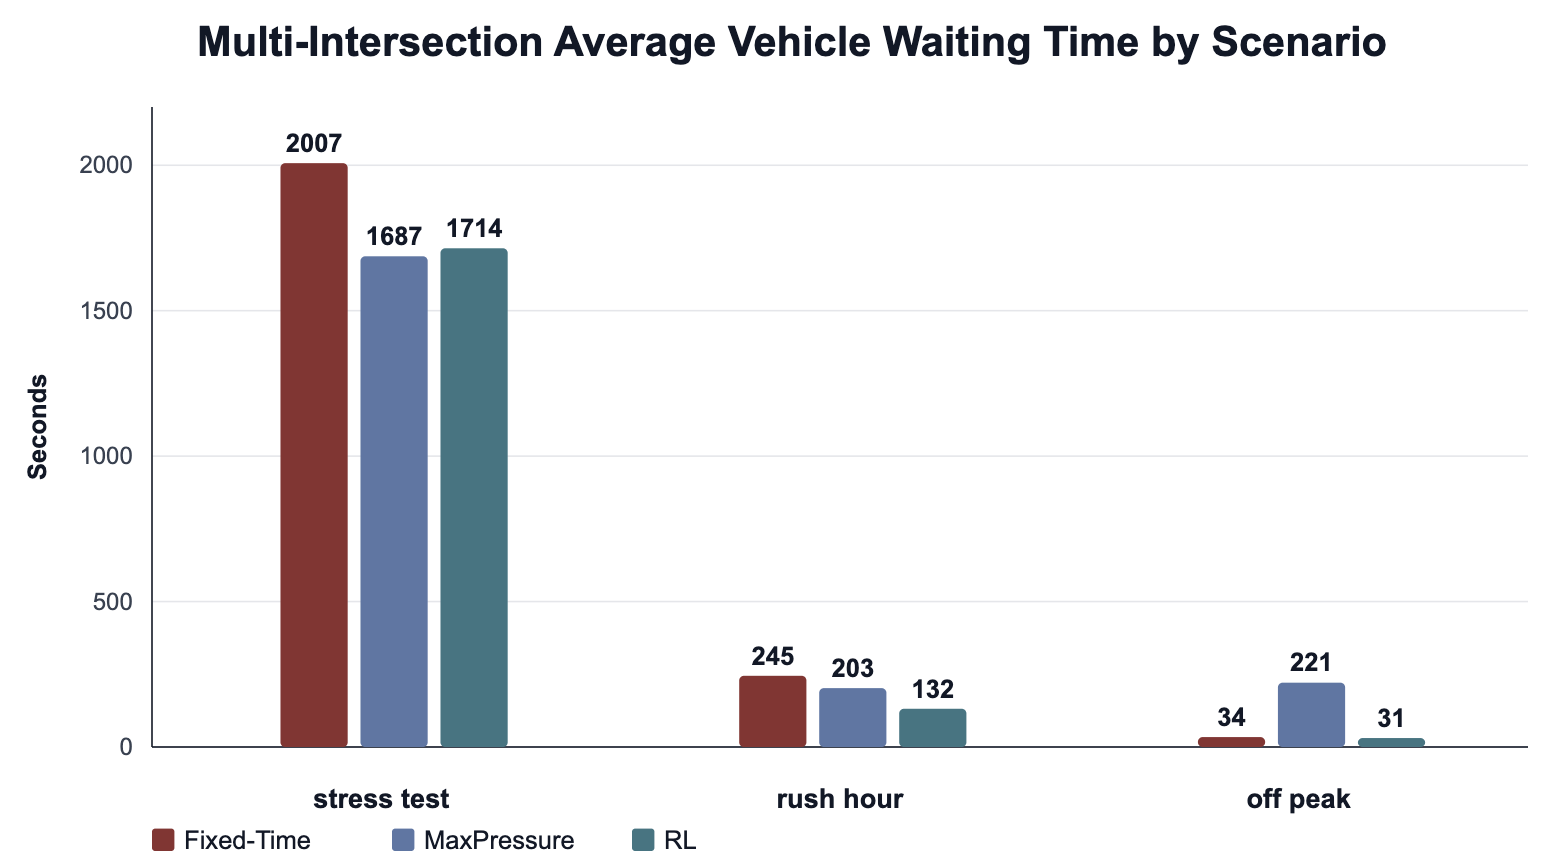
\includegraphics[width=0.48\textwidth]{img/evaluation_wait_by_scenario.png}
    \caption{Multi-Intersection Average Vehicle Waiting Time comparison between Fixed-Time, MaxPressure (rule-based), and the RL controller.}
    \label{fig:evaluation_wait_by_scenario}
\end{figure}

\section{Analysis and Validation}

The collected data demonstrates that the RL agent successfully moved away from rigid cyclical logic, favoring a responsive policy that prioritizes traffic based on real-time network pressure. At the single intersection, the 65.5\% reduction in maximum waiting time (falling from 139.0s to 48.0s) is particularly telling; it confirms that the agent effectively eliminated the "starvation" of minor approaches that typically plagues fixed-time schedules. Crucially, these efficiency gains were achieved without reducing overall throughput, confirming that the improvement stems from optimized signal timing rather than simply limiting network entry.

In the multi-intersection setup, performance gains were more modest (5.5--9.2\% improvement). This validates the expected difficulty of decentralized scaling; while the agents effectively managed local pressure, they lacked global awareness, occasionally leading to minor downstream bottlenecks. However, the comparison with the MaxPressure heuristic (Figure \ref{fig:evaluation_wait_by_scenario}) highlights the RL agent's value. In rush-hour scenarios, the RL agent achieved significantly lower wait times (132s) than MaxPressure (203s), suggesting that the agent's ability to learn non-linear phase-switching patterns makes it better suited for extreme traffic surges than simple rule-based heuristics.

The project objectives were met: the SUMO environment was accurately grounded in real-world topology, and the decentralized framework was validated against both static and heuristic baselines. A primary constraint of the study is the absolute reliance on synthesized demand generation. While the simulation is mapped using field-recorded turn restrictions, the demand files remain algorithmic proxies. They lack real-world nuances like unpredictable public transport stops, aggressive jaywalking, or uneven human lane adherence, all of which naturally disrupt theoretical traffic flow. Consequently, the RL agent may be over-optimized for the simulation environment, and true hardware-in-the-loop deployment would be the necessary next step to confirm these performance benefits on the physical Komitas corridor.

\section{Discussion and Conclusion}

This project successfully developed an authentic, field-grounded traffic simulation for the Komitas Avenue corridor and implemented a decentralized deep reinforcement learning framework to replace traditional fixed-time signaling. The primary contribution of this work is the demonstration that deep RL agents, trained with local observation vectors, can effectively manage complex, asymmetrical urban intersections without requiring a globally centralized controller. My findings indicate that while decentralized agents consistently outperform static baselines—achieving a 65.5\% reduction in maximum waiting time at isolated nodes and maintaining corridor-wide flow improvements of approximately 5--9\%—their local optimization patterns are highly effective yet distinct from the behavior of global systems.

A primary constraint of the study is the absolute reliance on synthesized demand generation. While the simulation is probabilistically mapped utilizing field turn restrictions, the demand files remain algorithmic proxies rather than actual localized induction-loop or optical camera data directly exported from the Yerevan municipality. Consequently, extreme bounds, such as the corridor stress scenario, might lack physical pavement nuances like unpredictable public transportation blocking, uneven human lane adherence, and heavy jaywalking impedance, which naturally disrupt theoretical mathematical flows. Validating deep performance would eventually require physical test-bench simulations or true hardware-in-the-loop deployment systems.

Future research should focus on implementing Multi-Agent Reinforcement Learning (MARL) architectures where adjacent agents can exchange "intent" signals or queue-state snapshots to mitigate downstream bottlenecks. In conclusion, the project objectives were fully achieved: the SUMO environment was accurately grounded in local geography, the phase-selection framework was successfully implemented, and the performance benefits of decentralized RL versus static traffic optimization were rigorously evaluated.

\appendices

\section{Supplementary Video}

A video demonstration of the simulation is available at:

\href{https://drive.google.com/file/d/1KRslnW8ghdw45RbBAjVVYINz5Oh-5XL_/view?usp=sharing}{Simulation Video}

\section*{Acknowledgment}
I sincerely thank my supervisor, Davit Ghazaryan, for his ongoing support and guidance throughout this project.
\vspace{1em}

\textit{Note: Gemini was used only for minor language editing, grammar refinement, and improving sentence coherence. The research design, implementation, analysis, results, and final content were independently developed, reviewed, and validated by the author.}

\bibliographystyle{IEEEtran}
\bibliography{references}

\end{document}
